\section{Experiment Design}	\label{sec:experiments}
	In this paper, five different scenarios in which two callers (peers) communicate using VoIP are considered to see the quality of calls made at a variety of distances. 
	
	In Scenario 1 (\hyperref[fig:scene-1]{Figure \ref{fig:scene-1}}), peer `A' (IP::10.127.10.203) and peer `B' (IP::10.127.204.227) are calling from within the same lab/office, which lets them connect to the same access point. Since both callers are at the same location, jitter can be expected to be very minimal and loss for of sent/received packets is the same at the both peers. In \hyperref[fig:scene-out-1]{Figure \ref{fig:scene-out-1}} it can be sees thaat the sending jitter at both peers have similar patterns. However, there jitter values differ; this could be due to differences between the devices. 
	\begin{figure}[tbh]
		\begin{minipage}{\textwidth}
%			\vspace{2mm}
			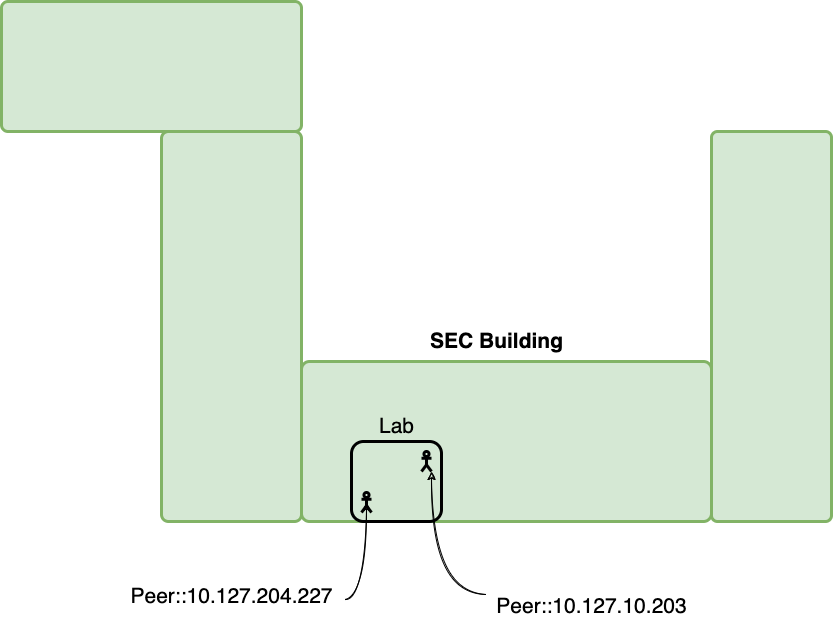
\includegraphics[scale=0.29]{Images/experiment/senarios/in_lab.drawio.png}
%			\vspace{2mm}
		\end{minipage}
		\caption{Scenario 1: Two peers within same office}
		\label{fig:scene-1}
	\end{figure}

	\begin{figure}[!b]
		\begin{minipage}{\textwidth}
			%			\vspace{2mm}
			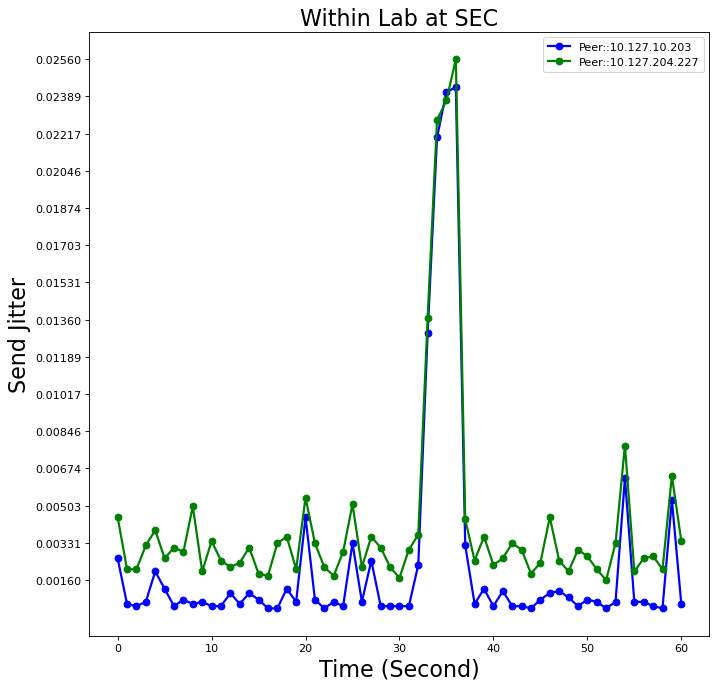
\includegraphics[scale=0.38]{Images/experiment/senarios/df_in_lab.png}
			%			\vspace{2mm}
		\end{minipage}
		\caption{Jitter values for the time spent by callers (for Scenario 1)}
		\label{fig:scene-out-1}
	\end{figure}


	In Scenario 2 (\hyperref[fig:scene-2]{Figure \ref{fig:scene-2}}), peer `A' (IP::10.127.10.203) and peer `B' (IP::10.127.204.227) are calling from different locations. Peer `A' is staying at the same lab/office seen in Scenario 1 and peer `B' is continuously moving to different locations while remaining at the same floor in the same building as peer `A'. This can let peer `B' change its access point within same local area network. Now, here we can expect that peer `B' will have more jitter then peer `A', since peer `B' has to connect and re-connect to different access points. \hyperref[fig:scene-out-2]{Figure \ref{fig:scene-out-2}} it can be seen the sending jitter at both peers have almost same patterns and differences as Scenario 1. However, since peer `B' is moving from one location to another, two peaks in the charted jitter of peer 'B' appear which are far higher than seen with peer `A' at the same point in time, which could appear when peer 'B' connects to a new access point and/or re-connects to a previous access point.
	\begin{figure}[tbh]
		\begin{minipage}{\textwidth}
			%			\vspace{2mm}
			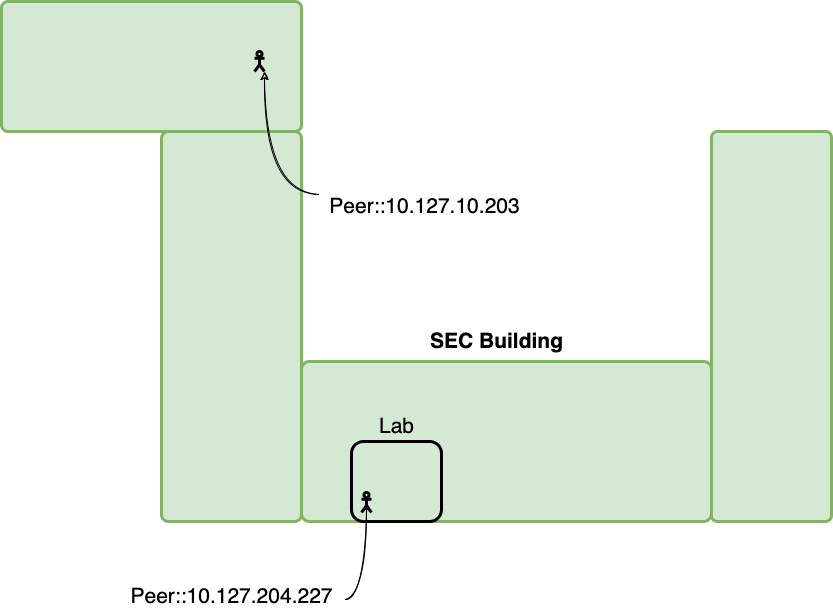
\includegraphics[scale=0.29]{Images/experiment/senarios/in_floor.drawio.png}
			%			\vspace{2mm}
		\end{minipage}
		\caption{Scenario 2: Two peers within same floor}
		\label{fig:scene-2}
	\end{figure}

	\begin{figure}[!b]
		\begin{minipage}{\textwidth}
			%			\vspace{2mm}
			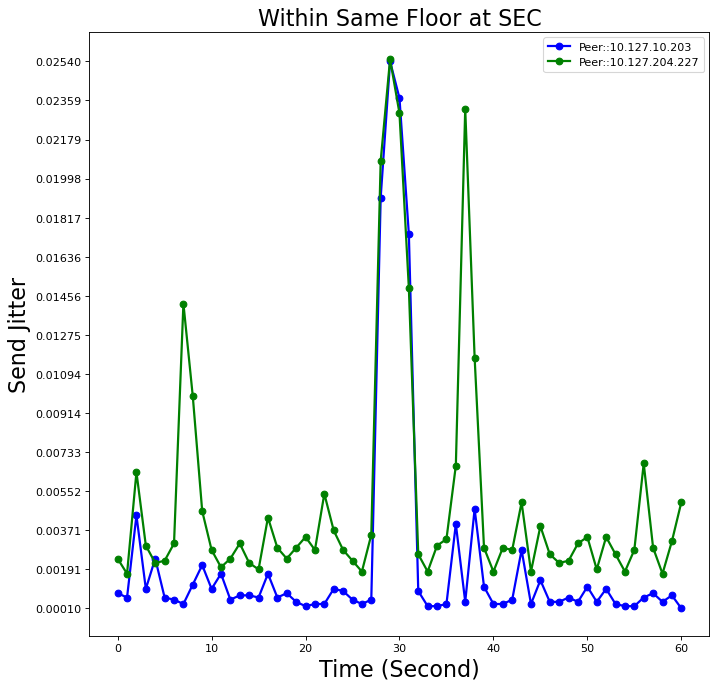
\includegraphics[scale=0.38]{Images/experiment/senarios/df_in_floor.png}
			%			\vspace{2mm}
		\end{minipage}
		\caption{Jitter values for the time spent by callers (for Scenario 2)}
		\label{fig:scene-out-2}
	\end{figure}

	In Scenario 3 (\hyperref[fig:scene-3]{Figure \ref{fig:scene-3}}), peer `A' (IP::10.127.10.203) and peer `B' (IP::10.127.204.227) are calling from different locations. Peer `A' is staying at same lab/office seen in Scenario 1 and peer `B' is continuously moving to different locations within the same building, but never on same floor. It is expected that peer `B' will have more jitter then peer `A', as peer `B' has to connect and re-connect to different access points. \hyperref[fig:scene-out-3]{Figure \ref{fig:scene-out-3}} we can see the sending jitter at both peers have almost same patterns and differences as Scenario 1. However, since peer `B' is moving from one location to another, many peaks appear which are much higher than those seen with peer `A', which could appear when peer 'B' connects to a new access point and/or re-connects to a previous access point.
	\begin{figure}[thb]
		\begin{minipage}{\textwidth}
			%			\vspace{2mm}
			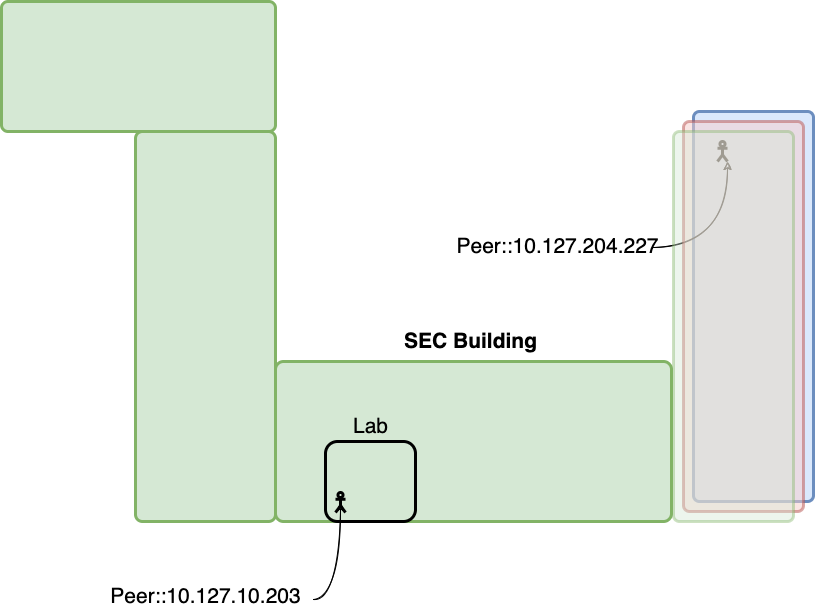
\includegraphics[scale=0.29]{Images/experiment/senarios/diff_floor.drawio.png}
			%			\vspace{2mm}
		\end{minipage}
		\caption{Scenario 3: Two peers at different floors but within the same building}
		\label{fig:scene-3}
	\end{figure}

	\begin{figure}[!b]
		\begin{minipage}{\textwidth}
			%			\vspace{2mm}
			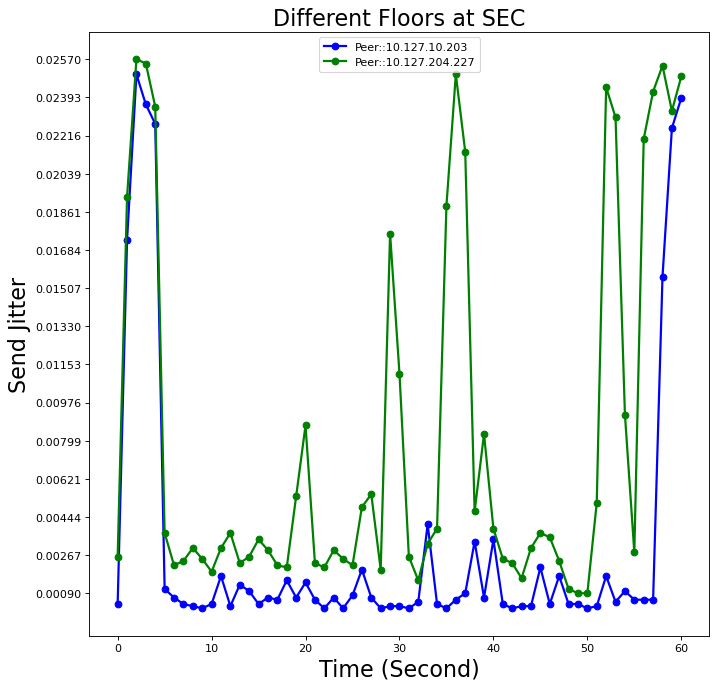
\includegraphics[scale=0.38]{Images/experiment/senarios/df_diff_floor.png}
			%			\vspace{2mm}
		\end{minipage}
		\caption{Jitter values for the time spend by callers (for Scenario 3)}
		\label{fig:scene-out-3}
	\end{figure}


	In Scenario 4 (\hyperref[fig:scene-4]{Figure \ref{fig:scene-4}}), peer `A' (IP::10.127.10.203) and peer `B' (IP::10.127.204.227) are calling from different locations. Peer `A' is staying at same lab/office seen in Scenario 1 and peer `B' is continuously moving outside of the same building as the lab where peer 'A' resides. This will allow peer `B' to be close to the same access point as peer 'A', but much farther from it. It can be expected that peer `B' will have more jitter then peer`A', since peer `B' has to connect and re-connect to different access points. At one point peer `B' disconnects from the network, which led to the call being terminated early and a lack of additional jitter data following the disconnection. In \hyperref[fig:scene-out-4]{Figure \ref{fig:scene-out-4}} it can be seen the sending jitter at both peers have almost same patterns and differences as Scenario 1. However, since peer `B' is moving one location to another, many peaks appear which are much higher than those seen with peer `A', which could appear when peer 'B' connects to a new access point and/or re-connects to a previous access point.
	\begin{figure}[thb]
		\begin{minipage}{\textwidth}
			%			\vspace{2mm}
			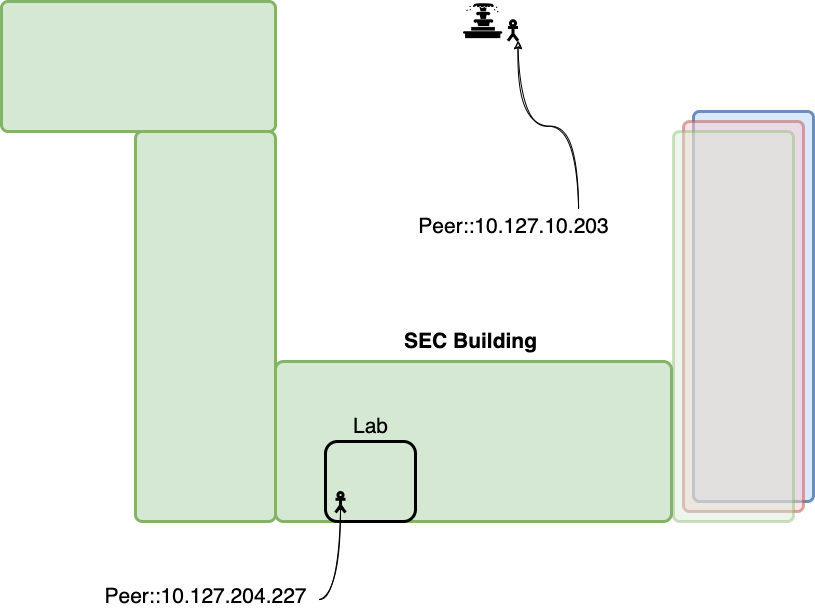
\includegraphics[scale=0.29]{Images/experiment/senarios/near_fountain.drawio.png}
			%			\vspace{2mm}
		\end{minipage}
		\caption{Scenario 4: Two peers are at different locations but close access points}
		\label{fig:scene-4}
	\end{figure}

	\begin{figure}[!b]
		\begin{minipage}{\textwidth}
			%			\vspace{2mm}
			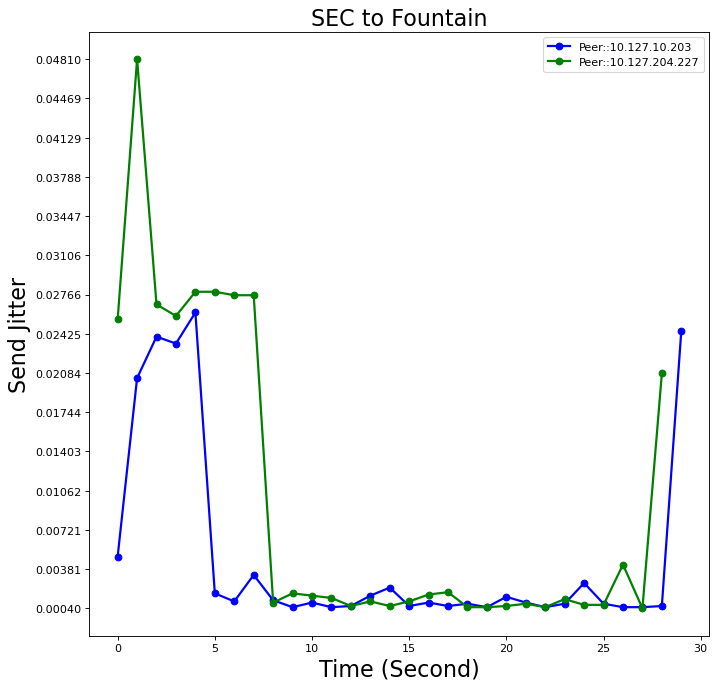
\includegraphics[scale=0.38]{Images/experiment/senarios/df_fountain.png}
			%			\vspace{2mm}
		\end{minipage}
		\caption{Jitter values for the time spent by callers (for Scenario 4)}
		\label{fig:scene-out-4}
	\end{figure}


	In Scenario 5 (\hyperref[fig:scene-5]{Figure \ref{fig:scene-5}}), peer `A' (IP::10.127.10.203) and peer `B' (IP::10.127.204.227) are calling from different locations. Peer `A' is staying at same lab/office as seen in Scenario 1 and peer `B' is continuously moving within a different building. It can be expected that peer `B' will have more jitter then peer`A', since peer `B' has to connect and re-connect to different access points. In \hyperref[fig:scene-out-5]{Figure \ref{fig:scene-out-5}} it can be seen the sending jitter at both peers have almost same patterns and differences as Scenario 1. However, since peer `B' is moving one location to another, many peaks appear which are much higher than those seen with peer `A', which could appear when peer 'B' connects to a new access point and/or re-connects to a previous access point.
	\begin{figure}[tbh]
		\begin{minipage}{\textwidth}
			%			\vspace{2mm}
			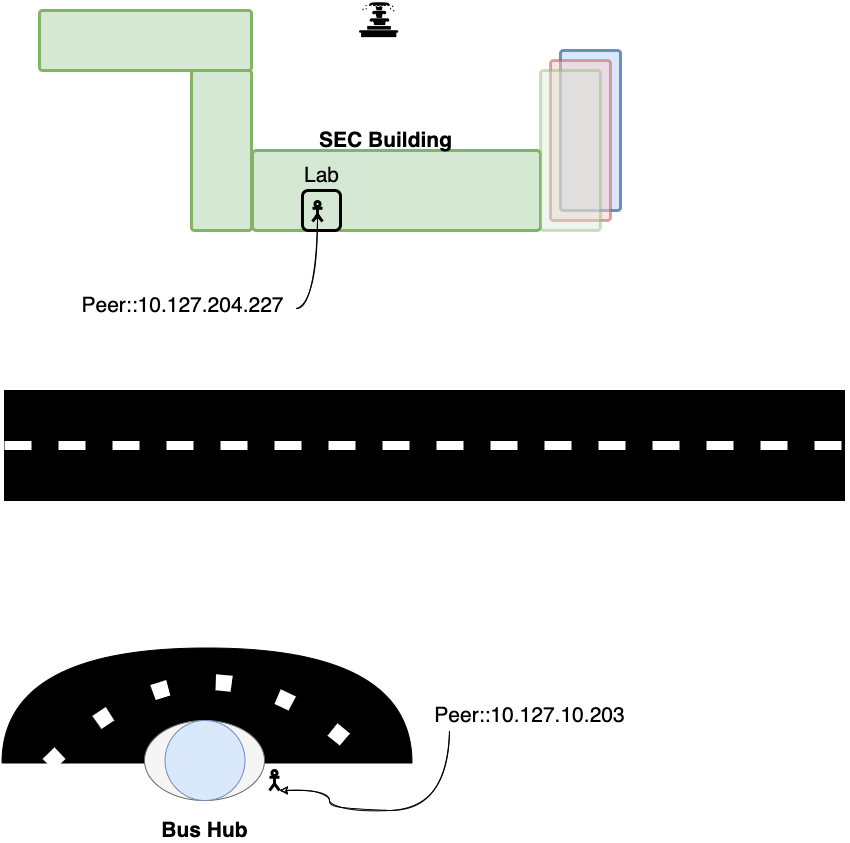
\includegraphics[scale=0.29]{Images/experiment/senarios/bus_hub.drawio.png}
			%			\vspace{2mm}
		\end{minipage}
		\caption{Scenario 5: Two peers are at different locations and different access points}
		\label{fig:scene-5}
	\end{figure}

	\begin{figure}[tbh]
		\begin{minipage}{\textwidth}
			%			\vspace{2mm}
			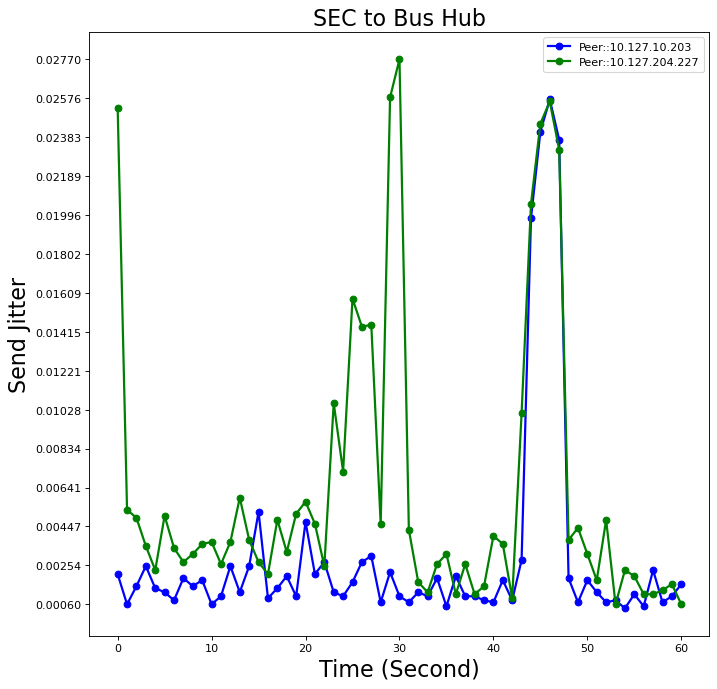
\includegraphics[scale=0.38]{Images/experiment/senarios/df_bus_hub.png}
			%			\vspace{2mm}
		\end{minipage}
		\caption{Jitter values for the time spent by callers (for Scenario 5)}
		\label{fig:scene-out-5}
	\end{figure}